\documentclass[11pt,a4paper]{article}
\usepackage{amsmath}
\usepackage{amsfonts}
\usepackage{amssymb}
\usepackage{graphicx}
\usepackage[margin=1in]{geometry}
\usepackage{hyperref}
\usepackage{listings}
\usepackage{xcolor}
\usepackage{algorithm}
\usepackage{algpseudocode}
\usepackage{cleveref}
\usepackage{caption}
\usepackage{subcaption}

\usepackage[backend=biber,style=numeric,sorting=nty]{biblatex}
\addbibresource{ref.bib}

\title{Mesoscopic Model: Computational Framework for Dynamics Study}
\author{Research Project}
\date{\today}

\begin{document}

\maketitle

\tableofcontents
\newpage

\section{Background}

\subsection{Ising Models}

The Ising model is a fundamental statistical mechanical model that describes the behavior of magnetic systems. For a two-dimensional square lattice with nearest-neighbor interactions, the Hamiltonian is given by:

\begin{equation}
H = -J \sum_{\langle i,j \rangle} \sigma_i \sigma_j - h \sum_i \sigma_i
\end{equation}

where $\sigma_i \in \{-1, +1\}$ are the spin variables, $J$ is the coupling strength, $h$ is the external magnetic field, and $\langle i,j \rangle$ denotes nearest-neighbor pairs.

\subsubsection{Critical Temperature}

The critical temperature $T_c$ is a fundamental parameter that determines the phase transition between ordered and disordered phases. We experimentally use $T_c = 1.0$ and $T_c = 4.0$.

\begin{equation}
T_c = \frac{2J}{k_B \ln(1 + \sqrt{2})} \approx \frac{2.269J}{k_B}
\end{equation}

where $k_B$ is the Boltzmann constant. This critical temperature separates two distinct phases:

\begin{itemize}
    \item \textbf{High temperature regime} ($T > T_c$): The system is in a \textit{disordered phase} where spins are randomly oriented, resulting in zero net magnetization. The system exhibits thermal fluctuations and short-range correlations.
    
    \item \textbf{Low temperature regime} ($T < T_c$): The system is in an \textit{ordered phase} where spins tend to align, leading to non-zero magnetization. The system exhibits long-range order and reduced thermal fluctuations.
    
    \item \textbf{Critical region} ($T \approx T_c$): The system undergoes a phase transition with critical phenomena, including diverging correlation lengths and power-law scaling behavior.
\end{itemize}

The temperature ratio $T/T_c$ is a key parameter that determines the physical regime of the system. In our simulations, we often work in the high-temperature regime where $T/T_c > 1$, corresponding to the disordered phase.

\subsubsection{Units and Normalization}

In our computational framework, we use dimensionless units where the Boltzmann constant $k_B = 1$ and the coupling strength $J = 1$. This normalization simplifies the calculations while preserving the essential physics. The temperature $T$ is therefore dimensionless, and the critical temperature becomes:

\begin{equation}
T_c = \frac{2}{\ln(1 + \sqrt{2})} \approx 2.269
\end{equation}

This approach is common in computational statistical physics as it eliminates the need to track physical units while maintaining the correct scaling relationships between temperature, energy, and other thermodynamic quantities.

In this normalization, the inverse temperature $\beta = 1/T$ is directly computed from the dimensionless temperature $T$. For example, with $T = 6.808$, we have $\beta = 1/6.808 \approx 0.147$, which represents the strength of thermal fluctuations in the system.

\subsection{Nonlocal Interactions and Kac Potentials}

The classical Ising model only considers nearest-neighbor interactions. 
However, many physical systems exhibit \emph{nonlocal interactions} that extend beyond immediate neighbors. 
To incorporate such effects, one introduces \emph{Kac-type potentials}, which are long-range interaction kernels that decay with distance.

A Kac potential $J_\gamma(x,y)$ is typically defined as a smooth, radially symmetric function that depends on a parameter $\gamma > 0$ controlling the interaction range:
\begin{equation}
    J_\gamma(x, y) = \gamma^{-d} J\left(\frac{|x - y|}{\gamma}\right),
\end{equation}
where $J(r)$ is a normalized kernel function, and $d$ is the spatial dimension. Larger values of $\gamma$ correspond to longer-range interactions, while smaller values approach the nearest-neighbor limit.

A widely used example of a Kac potential is the Gaussian kernel:
\begin{equation}\label{eq:J-Gaussian}
J_\gamma(x) \;=\; \frac{1}{(2\pi\gamma^2)^{d/2}} 
\exp\!\left(-\frac{|x|^2}{2\gamma^2}\right).
\end{equation}

The Ising Hamiltonian with Kac interactions is given by
\begin{equation}\label{eq:H-Kac}
    H(\sigma) \;=\; -\frac{1}{2}\sum_{x,y} J_\gamma(x,y)\,\sigma(x)\sigma(y) \;-\; h \sum_{x} \sigma(x).
\end{equation}

\subsection{Glauber Dynamics}
\label{sec:glauber}
To describe the stochastic time evolution of the spin system, we adopt \emph{Glauber dynamics}. 
At each site, spins flip randomly due to thermal fluctuations, with probabilities determined by the change in the Hamiltonian.

\paragraph{Spin-Flip Probability.}  
Let $\beta > 0$ be the inverse temperature. 
For a given spin $\sigma(x)$, the probability of flipping at site $x$ depends on the local field
\begin{equation}\label{eq:hloc}
    h_{\gamma}(x) \;=\; h + \sum_{y\neq x} J_\gamma(x-y)\,\sigma(y).
\end{equation}
The corresponding flip probability can be written in several equivalent forms:
\begin{equation}\label{eq:flip-prob}
\begin{split}
    P\big(\sigma(x)\!\to\!-\sigma(x)\big) 
    &= \frac{1}{1 + \exp\!\big(\beta \Delta H_x\big)} 
        \quad \text{(from energy difference)} \\
    &= \frac{1}{1 + \exp\!\big(2\beta\,\sigma(x) h_{\gamma}(x)\big)} 
        \quad \text{(logistic form)} \\
    &= \frac{\exp\!\big(-\beta\sigma(x) h_{\gamma}(x)\big)}
            {2\cosh\!\big(\beta h_{\gamma}(x)\big)} 
        \quad \text{(factorized form, cf.~Masi et al.\cite{de1994glauber})}.
\end{split}
\end{equation}
Here, $\Delta H_x = H(\sigma^x) - H(\sigma) = 2\sigma(x)h_\gamma(x)$ denotes the energy change when flipping the spin at $x$.

\paragraph{Initialization by Gaussian Random Field.}

\paragraph{Stochastic Simulation via Gillespie Algorithm.}  
The Glauber dynamics can be efficiently simulated using the Gillespie algorithm (\cref{alg:gillespie}), 
which generates statistically exact trajectories of continuous-time Markov processes. 
The procedure is:

\begin{enumerate}
    \item Compute the total flip rate 
    \[
        R = \sum_{x} P\big(\sigma(x)\!\to\!-\sigma(x)\big).
    \]
    \item Draw the next time increment $\Delta t$ from an exponential distribution with mean $1/R$.
    \item Select a site $x$ to flip with probability proportional to its individual rate.
    \item Update $\sigma(x)\mapsto -\sigma(x)$, recompute local fields if needed, and repeat.
\end{enumerate}

\begin{algorithm}[h!]
\caption{Gillespie Simulation of Glauber Dynamics}
\label{alg:gillespie}
\begin{algorithmic}[1]
\State Initialize spin configuration $\sigma$ and compute local fields $h_\gamma(x)$.
\While{simulation time $t < t_{\mathrm{end}}$}
    \State Compute total flip rate 
    \[
        R = \sum_{x} P\big(\sigma(x)\!\to\!-\sigma(x)\big).
    \]
    \State Sample time increment $\Delta t \sim \mathrm{Exp}(R)$.
    \State Select site $x$ with probability 
    \[
        \frac{P(\sigma(x)\!\to\!-\sigma(x))}{R}.
    \]
    \State Flip spin: $\sigma(x) \gets -\sigma(x)$.
    \State Update local fields $h_\gamma(y)$ if needed.
    \State Advance time: $t \gets t + \Delta t$.
\EndWhile
\end{algorithmic}
\end{algorithm}
This algorithm gives an implementation of the Gillespie method for Glauber dynamics, ensuring accurate simulation of the spin system's stochastic behavior.

\paragraph{Stochastic Simulation via $\tau$-leaping Approximation.} The Gillespie algorithm simulates one event at a time, which can be slow for large systems. 
The \emph{$\tau$-leaping} method accelerates the simulation by leaping over a fixed time step $\tau$. 
During this interval, event rates are assumed to be constant. 
The number of events at each site is then sampled from a Poisson distribution. 
This allows many events to be processed in parallel.

\begin{algorithm}[h]
\caption{$\tau$-leaping for Glauber dynamics}
\begin{algorithmic}[1]
\State Initialize spins $s$, time $t=0$
\While{$t < T_{\text{end}}$}
    \State Compute local field $h_{\text{loc}}$
    \State Compute flip rates $r_i = \frac{1}{1 + \exp(2 \beta h_{\text{loc},i} s_i)}$
    \State Choose $\tau = \epsilon / \max_i r_i$
    \State Sample $K_i \sim \mathrm{Poisson}(r_i \tau)$
    \State Update spins: if $K_i$ is odd, flip $s_i$
    \State $t \gets t + \tau$
\EndWhile
\end{algorithmic}
\end{algorithm}

\paragraph{Comparison of Gillespie and $\tau$-leaping} We compare the two methods within a small lattice ($L=128$) to validate the $\tau$-leaping approximation. We use the same initial conditions and parameters for both simulations, and for each method, we run 20 independent trials to account for stochastic variability.

\section{PDE}

\subsection{Hydrodynamic Limit for Glauber-Kac}

Starting from the Glauber dynamics introduced in \cref{sec:glauber}, we consider the lattice in $[0,1]^d$. When the lattice size tends to infinity $L\to\infty$, and the empirical magnetization field
\begin{equation}
    m^L(t,\mathbf{x}) = \frac{1}{B^d}\sum_{z\in \Lambda_B(\mathbf{x})} \sigma_t(z)
\end{equation}
is coarse-grained over mesoscopic blocks of size $B$, the law of large numbers implies convergence of $m^L(t,\mathbf{x})$ to a deterministic limit $m(t,\mathbf{x})$. 
In this hydrodynamic limit, the Glauber dynamics is described by the nonlinear nonlocal PDE
\begin{equation}\label{eq:nonlocal}
    \partial_t m(t,\mathbf{x}) \;=\; -\,m(t,\mathbf{x})\;+\;\tanh\!\Big(\beta\, (J_\gamma * m)(t,\mathbf{x}) + \beta h\Big), 
    \qquad m(0,\mathbf{x})=m_0(\mathbf{x}),
\end{equation}
where the convolution operator is defined by
\begin{equation}
    \label{eq:convolution}
    (J_\gamma * m)(\mathbf{x}) \;=\; \int_{\mathbb{T}^d} J_\gamma(\mathbf{x},\mathbf{y})\,m(\mathbf{y})\,d\mathbf{y}.
\end{equation}

Equation~\eqref{eq:nonlocal} is the mesoscopic limit of the Glauber--Kac dynamics: 
the microscopic randomness averages out, and the macroscopic magnetization evolves deterministically according to a nonlocal reaction term given by the Kac potential.

\subsection{From the Nonlocal to the Local PDE}
Assume $m$ is smooth on the scale of $\gamma$, we can perform a Taylor expansion of the convolution term in \cref{eq:convolution}:
\begin{equation}
    (J_\gamma * m)(\mathbf{x}) = m(\mathbf{x}) + \frac{\gamma^2}{2}\Delta m(\mathbf{x}) + O(\gamma^4).
\end{equation}

Also, we can expand $\tanh$ in \cref{eq:nonlocal} around $m(\mathbf{x}) + h$:
\begin{equation}
    \tanh(\beta u) = \beta u - \frac{(\beta u)^3}{3} + O(u^5).
\end{equation}

Substituting these expansions into \cref{eq:nonlocal} and neglecting higher-order terms, we obtain the local reaction-diffusion PDE:
\begin{equation}\label{eq:local}
    \partial_t m(t,\mathbf{x}) = \kappa \Delta m(t,\mathbf{x}) - f(m(t,\mathbf{x})) + \beta h,
    \qquad m(0,\mathbf{x})=m_0(\mathbf{x}),
\end{equation}
where the effective diffusion coefficient is given by
\begin{equation}
    \kappa = \beta \frac{m_2}{2d} \gamma^2,
\end{equation}
with $m_2 = \int_{\mathbb{R}^d} |x|^2 J(x) dx$ being the second moment of the kernel $J$. And the reaction term is
\begin{equation}
    f(m) = -rm - u m^3 + \text{higher order terms}, \quad r = 1-\beta, \quad u = \frac{\beta^3}{3}.
\end{equation} 


\section{Experimental Settings}

\subsection{Parameter Configuration}

Our computational experiments are designed to systematically explore the parameter space of the Ising model and its mesoscopic approximations. The base configuration uses:

\begin{itemize}
    \item \textbf{Coupling strength}: $J = 1.0$ (dimensionless units)
    \item \textbf{Critical temperature}: $T_c = 2.27$ (for 2D square lattice)
    \item \textbf{Lattice size}: $L = 1024$ with coarse-graining to $M = 128$
    \item \textbf{Block size}: $B = 8$ (coarse-graining ratio $L/M = 8$)
    \item \textbf{Spatial resolution}: $\delta = 1/M = 0.0078125$
\end{itemize}

\subsubsection{Temperature Regimes}

We investigate two distinct temperature regimes:

\begin{enumerate}
    \item \textbf{Low temperature} ($T = 1.0$): Below critical temperature, corresponding to the ordered phase where $T/T_c \approx 0.44$
    \item \textbf{High temperature} ($T = 4.0$): Above critical temperature, corresponding to the disordered phase where $T/T_c \approx 1.76$
\end{enumerate}

\subsubsection{External Field Variations}

The external magnetic field $h$ is varied across four values to study its effect on the system dynamics:

\begin{itemize}
    \item $h = 0.0$ (no external field)
    % \item $h = 0.5$ (weak external field)
    \item $h = 1.0$ (moderate external field)
    % \item $h = 2.0$ (strong external field)
\end{itemize}

\subsubsection{Kernel Range Studies}

To investigate the role of interaction range in nonlocal dynamics, we vary the kernel domain size:

\begin{itemize}
    \item \textbf{Local interactions}: $\gamma \to 0$ (nearest-neighbor only)
    \item \textbf{Short-range nonlocal}: $\gamma = 2\delta$ (extended local interactions)
    \item \textbf{Medium-range nonlocal}: $\gamma = 4\delta$ (moderate nonlocal interactions)
\end{itemize}

This systematic variation allows us to study the transition from local to nonlocal behavior and its impact on pattern formation and dynamics.

This computational framework will provide insights into:

\begin{itemize}
    \item The relationship between microscopic and macroscopic dynamics
    \item The validity of continuum approximations
    \item The role of nonlocal interactions in pattern formation
    \item Machine learning approaches for complex dynamics
\end{itemize}

\subsection{Data v.s. PDE Solutions}
We compare the original data generated by \Cref{alg:gillespie} and PDE solutions under different settings.
\begin{table}[h]
    \centering
    \begin{tabular}{llll}
        \hline
        \hline
        \textbf{External field $h$} & \textbf{Temperature $T$} & \textbf{Kernel parameter $\gamma$} & \textbf{Results} \\
        \hline
        0 & 1 & 0.015625 & \Cref{fig:pde_comparison_h0_T1_eps0.015625} \\
        0 & 4 & 0.015625 & \Cref{fig:pde_comparison_h0_T4_eps0.015625} \\
        1 & 1 & 0.015625 & \Cref{fig:pde_comparison_h1_T1_eps0.015625} \\
        1 & 4 & 0.015625 & \Cref{fig:pde_comparison_h1_T4_eps0.015625} \\
        0 & 1 & 0.03125  & \Cref{fig:pde_comparison_h0_T1_eps0.03125}  \\
        0 & 4 & 0.03125  & \Cref{fig:pde_comparison_h0_T4_eps0.03125}  \\
        1 & 1 & 0.03125  & \Cref{fig:pde_comparison_h1_T1_eps0.03125}  \\
        1 & 4 & 0.03125  & \Cref{fig:pde_comparison_h1_T4_eps0.03125}  \\
        \hline
        \hline
    \end{tabular}
    \caption{Comparison of original data and PDE solutions under different external field $h$, temperature $T$, and kernel parameter $\epsilon$.}
    \label{tab:pde_comparison}
\end{table}

We present the results in \Cref{tab:pde_comparison}. The arrangement of the figure follows a $2 \times 4$ grid layout to clearly compare the original data and the PDE solutions. 
In the \textbf{top row}, the first two panels show the original data at the initial state ($t=0$) and at the final state ($t=5.0$). 
The third panel presents the magnetization evolution over time, comparing the original data with the nonlocal PDE solution, 
while the fourth panel shows the free energy evolution for both cases. 
In the \textbf{bottom row}, the first two panels display the nonlocal PDE solution at $t=0$ and $t=5.0$. 
The third panel gives the absolute difference (PDE$-$Data) at the final time, 
and the last panel illustrates the phase area fraction (fraction of $m>0$) as a function of time. 


% with epsilon = 0.015625

\begin{figure}[!h]
    \centering
    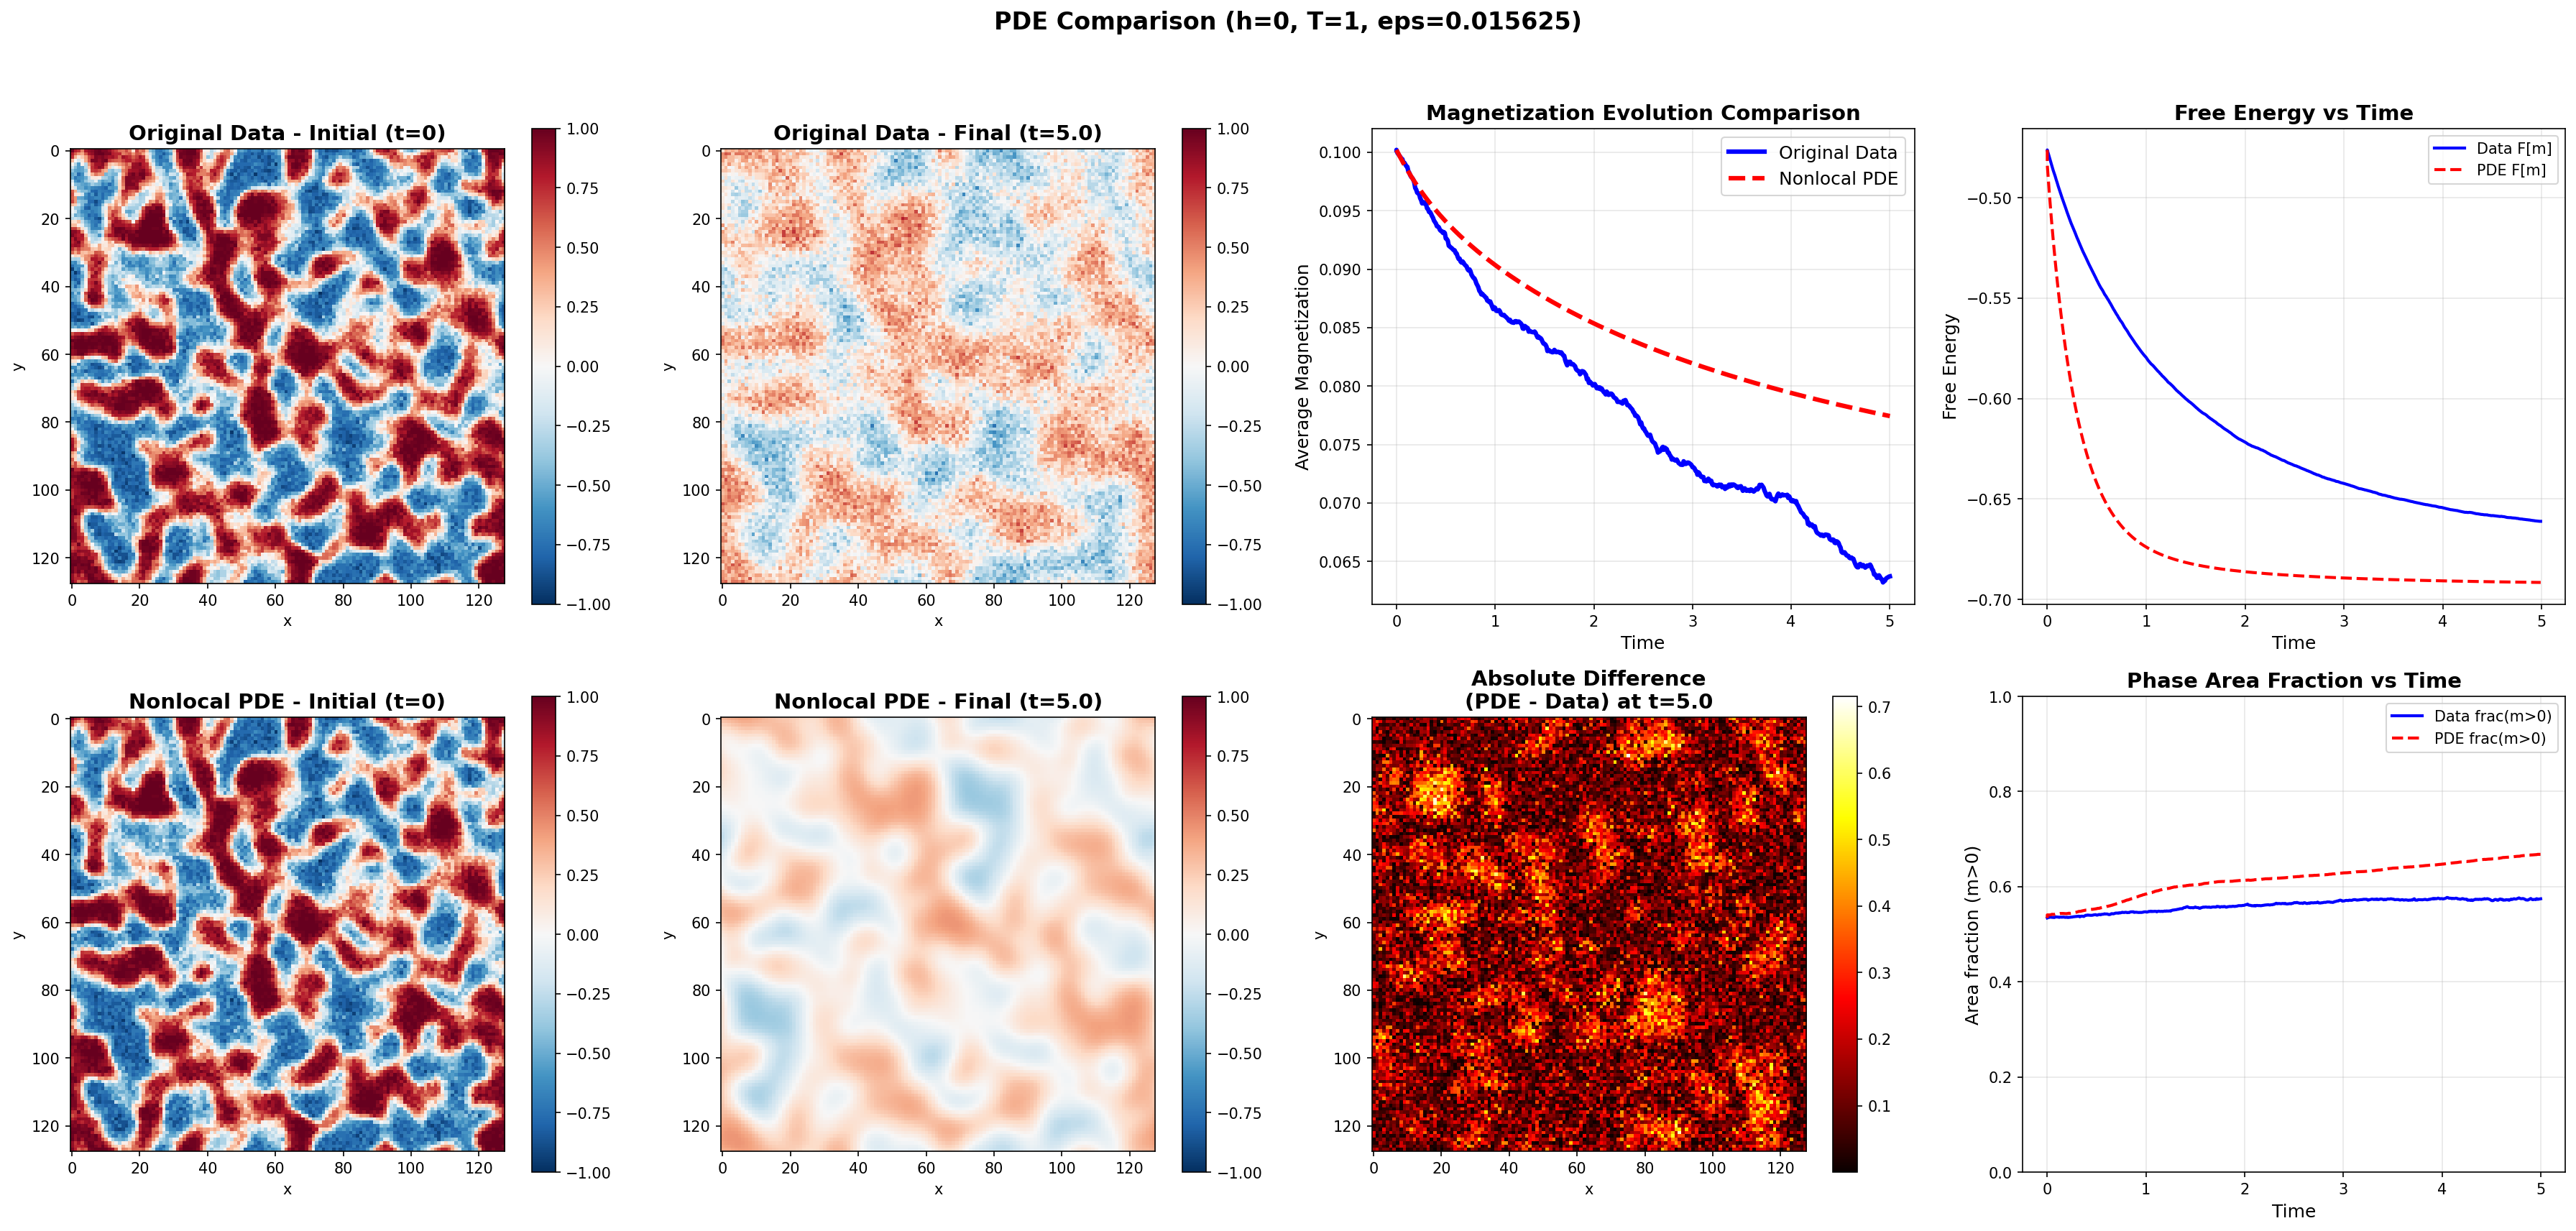
\includegraphics[width=1.0\textwidth]{fig/pde_comparison_h0_T1_eps0.015625.png}
    \caption{Comparison of original data and PDE solutions for $h=0$, $T=1$, $\epsilon=0.015625$.}
    \label{fig:pde_comparison_h0_T1_eps0.015625}
\end{figure}


\begin{figure}[!h]
    \centering
    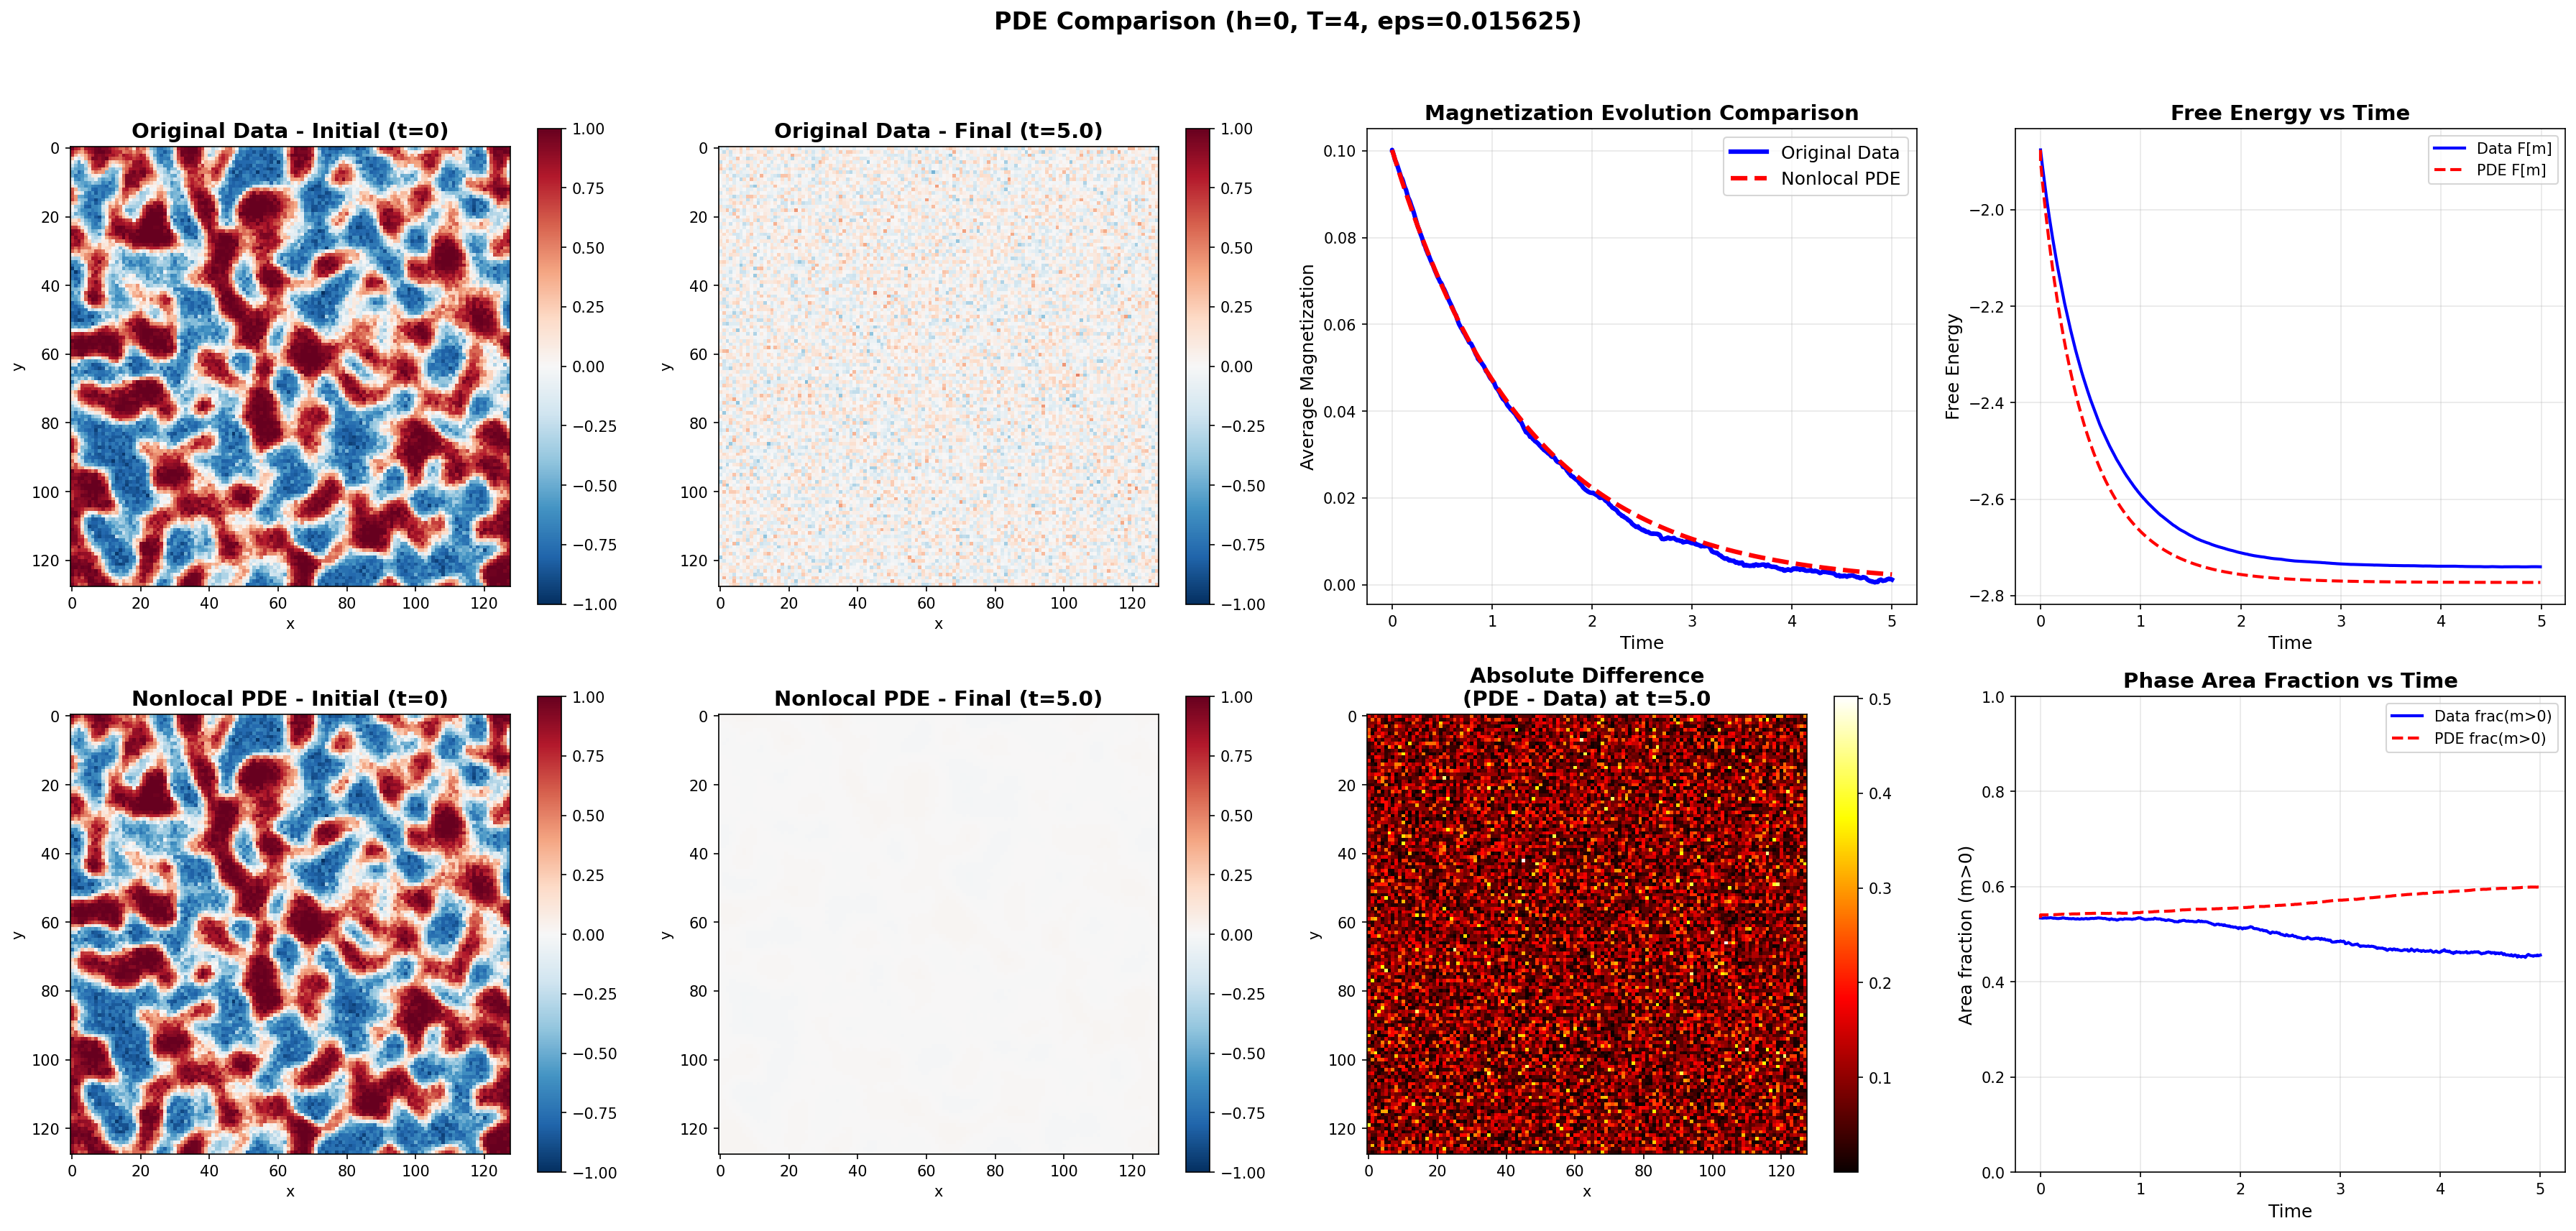
\includegraphics[width=1.0\textwidth]{fig/pde_comparison_h0_T4_eps0.015625.png}
    \caption{Comparison of original data and PDE solutions for $h=0$, $T=4$, $\epsilon=0.015625$.}
    \label{fig:pde_comparison_h0_T4_eps0.015625}
\end{figure}


\begin{figure}[!h]
    \centering
    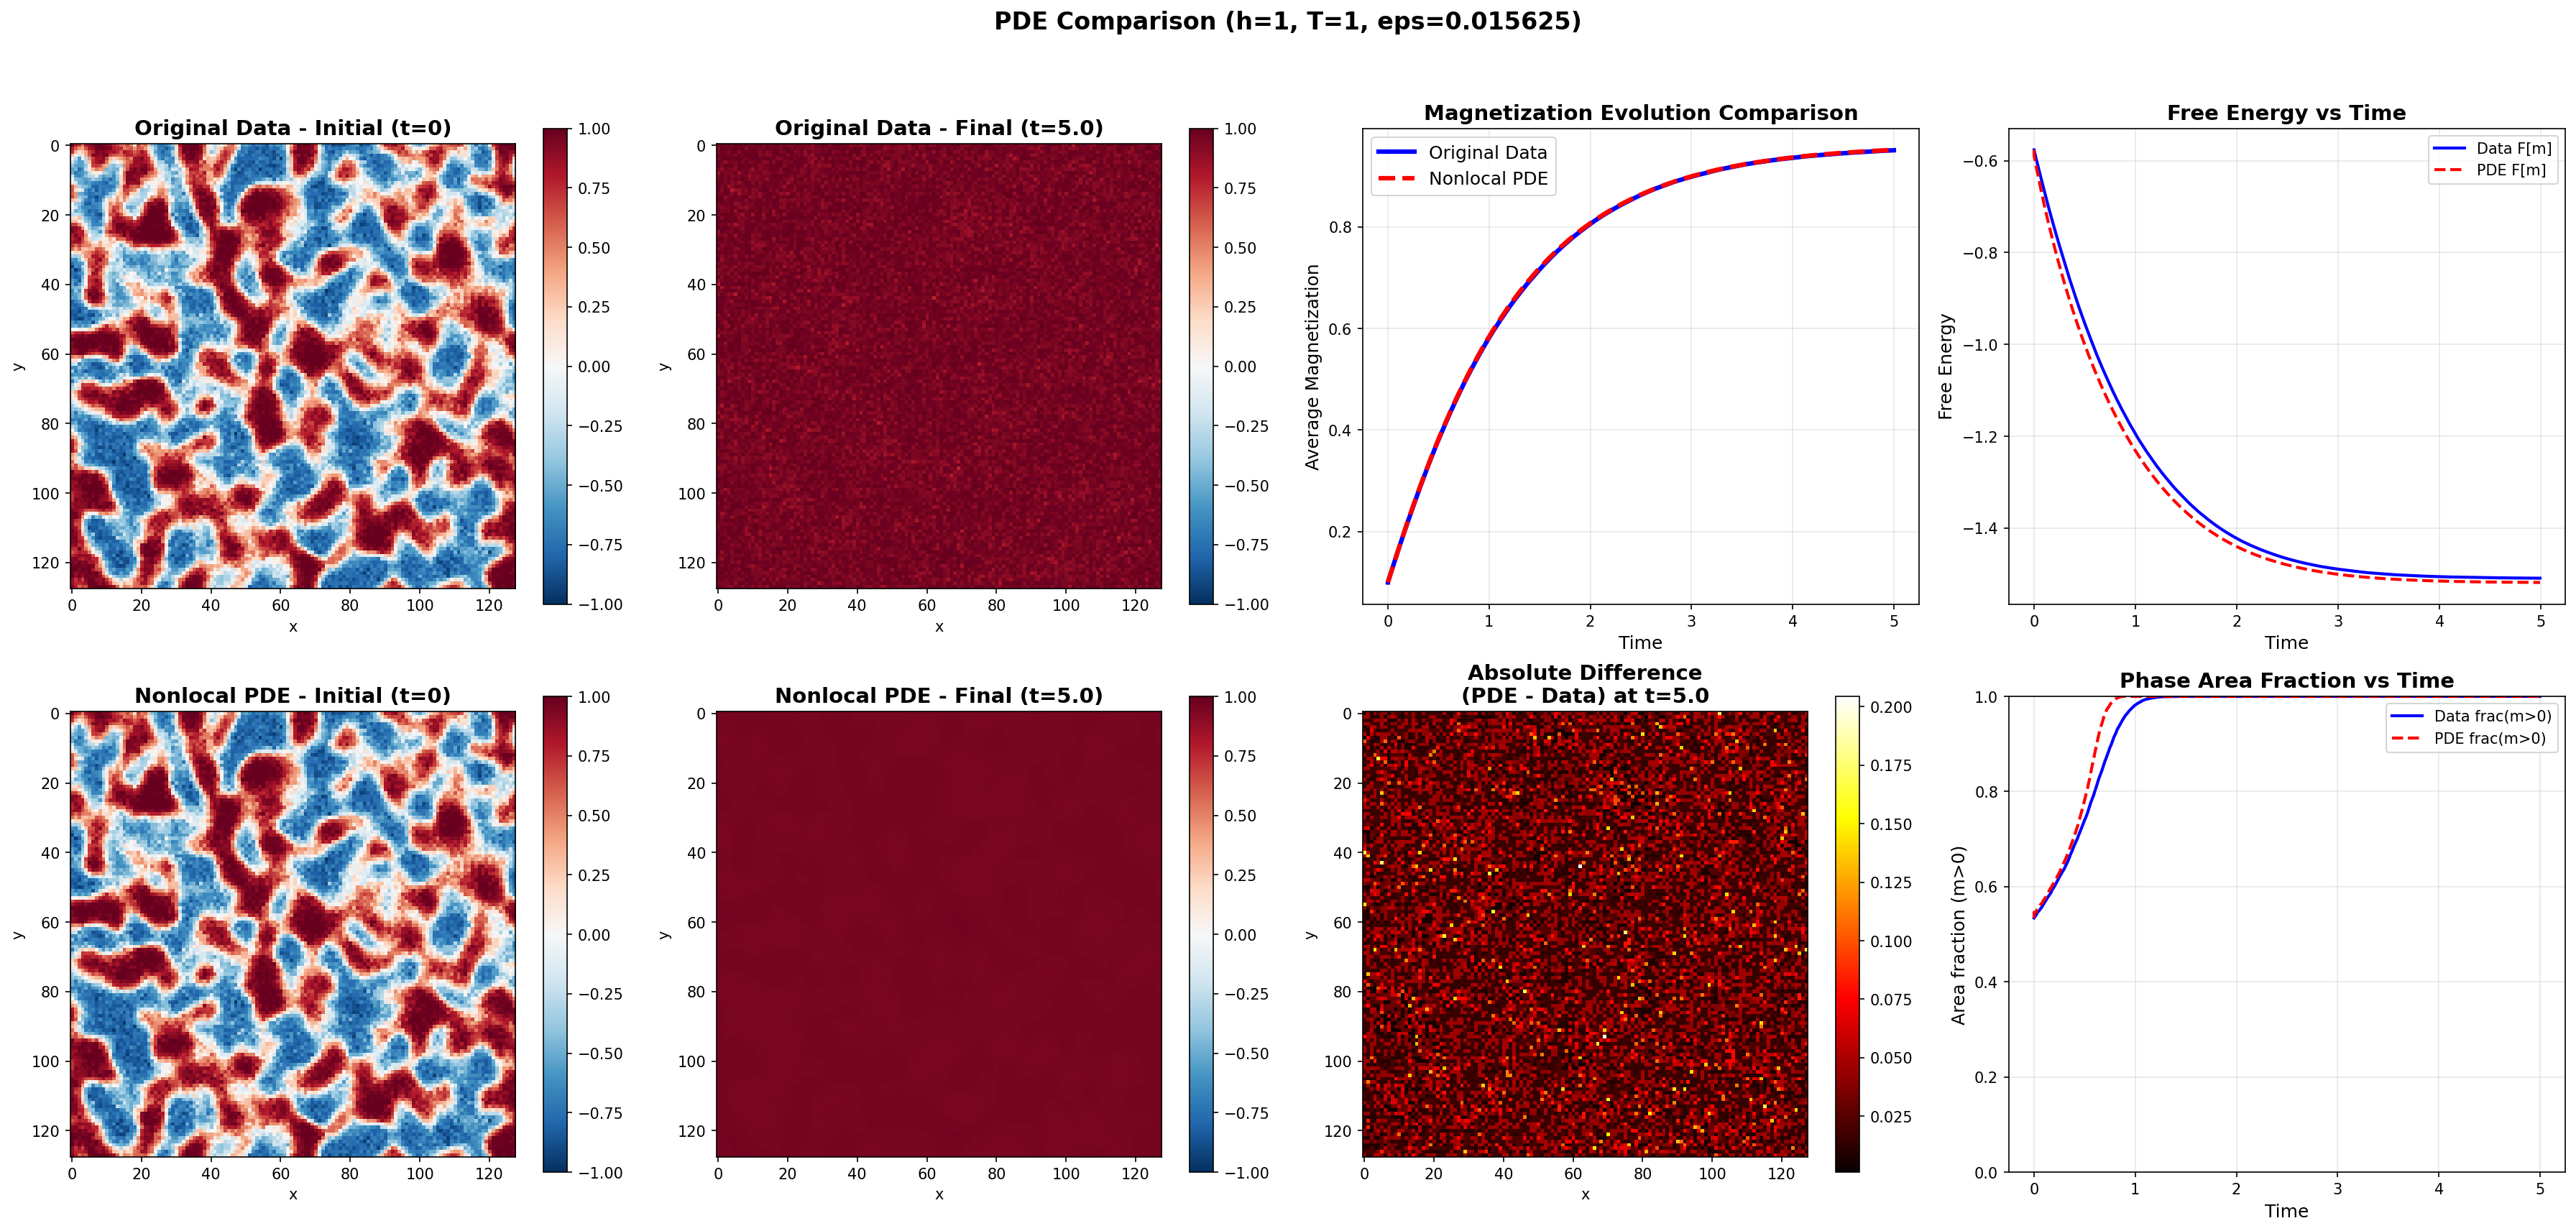
\includegraphics[width=1.0\textwidth]{fig/pde_comparison_h1_T1_eps0.015625.png}
    \caption{Comparison of original data and PDE solutions for $h=1$, $T=1$, $\epsilon=0.015625$.}
    \label{fig:pde_comparison_h1_T1_eps0.015625}
\end{figure}


\begin{figure}[!h]
    \centering
    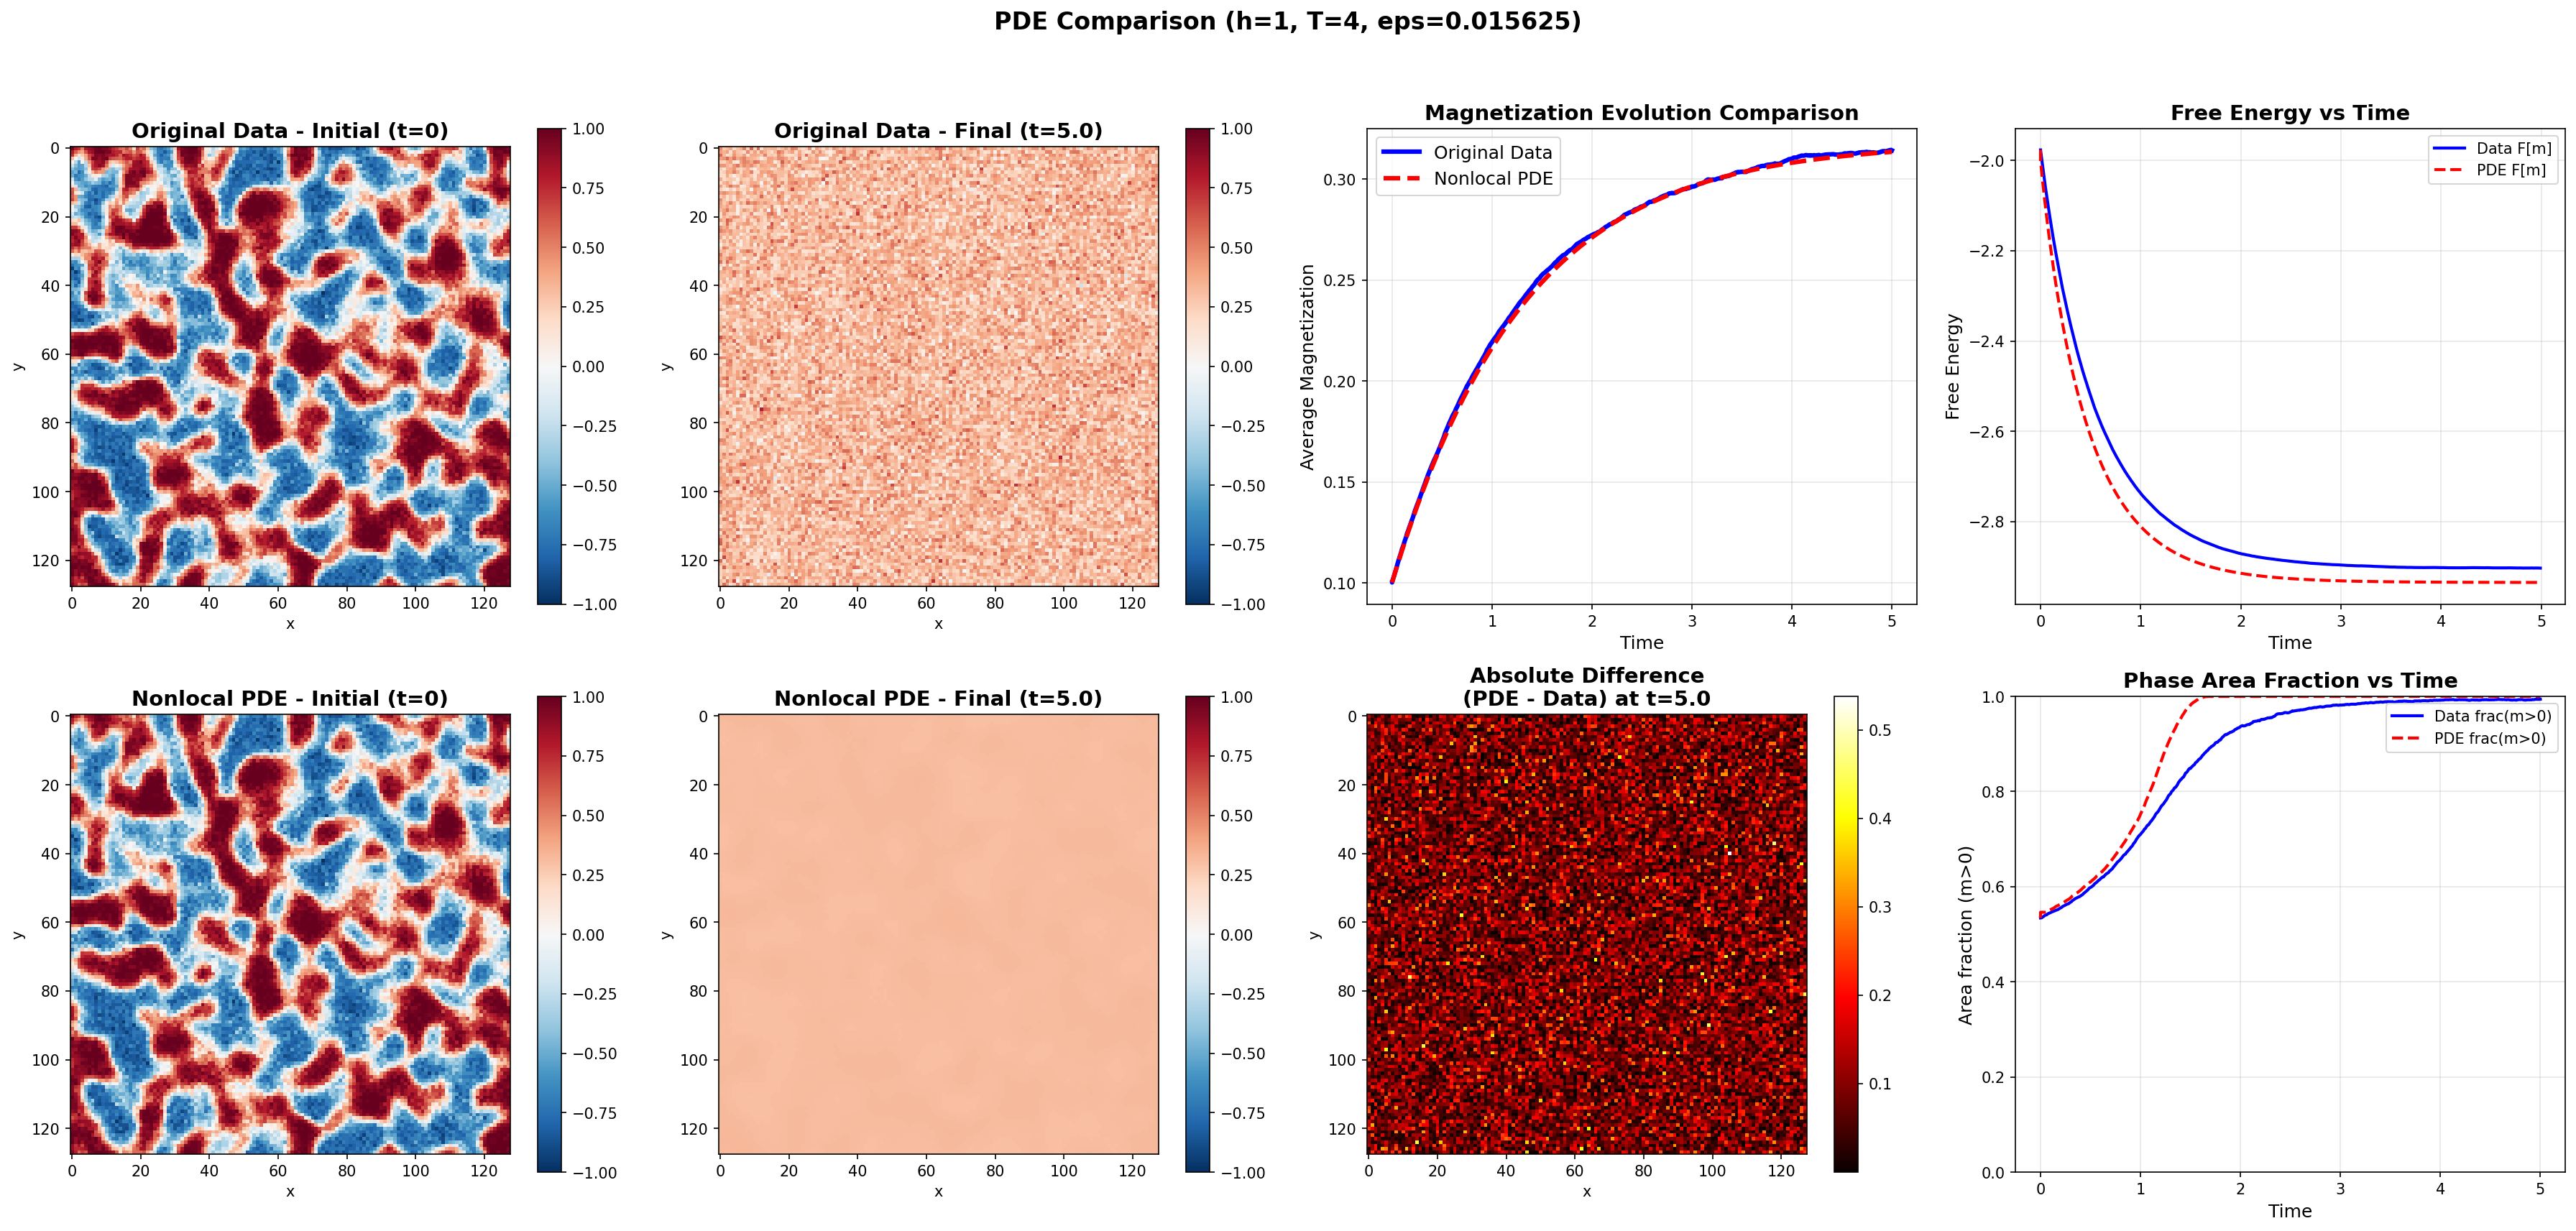
\includegraphics[width=1.0\textwidth]{fig/pde_comparison_h1_T4_eps0.015625.png}
    \caption{Comparison of original data and PDE solutions for $h=1$, $T=4$, $\epsilon=0.015625$.}
    \label{fig:pde_comparison_h1_T4_eps0.015625}
\end{figure}

% with epsilon = 0.03125

\begin{figure}[!h]
    \centering
    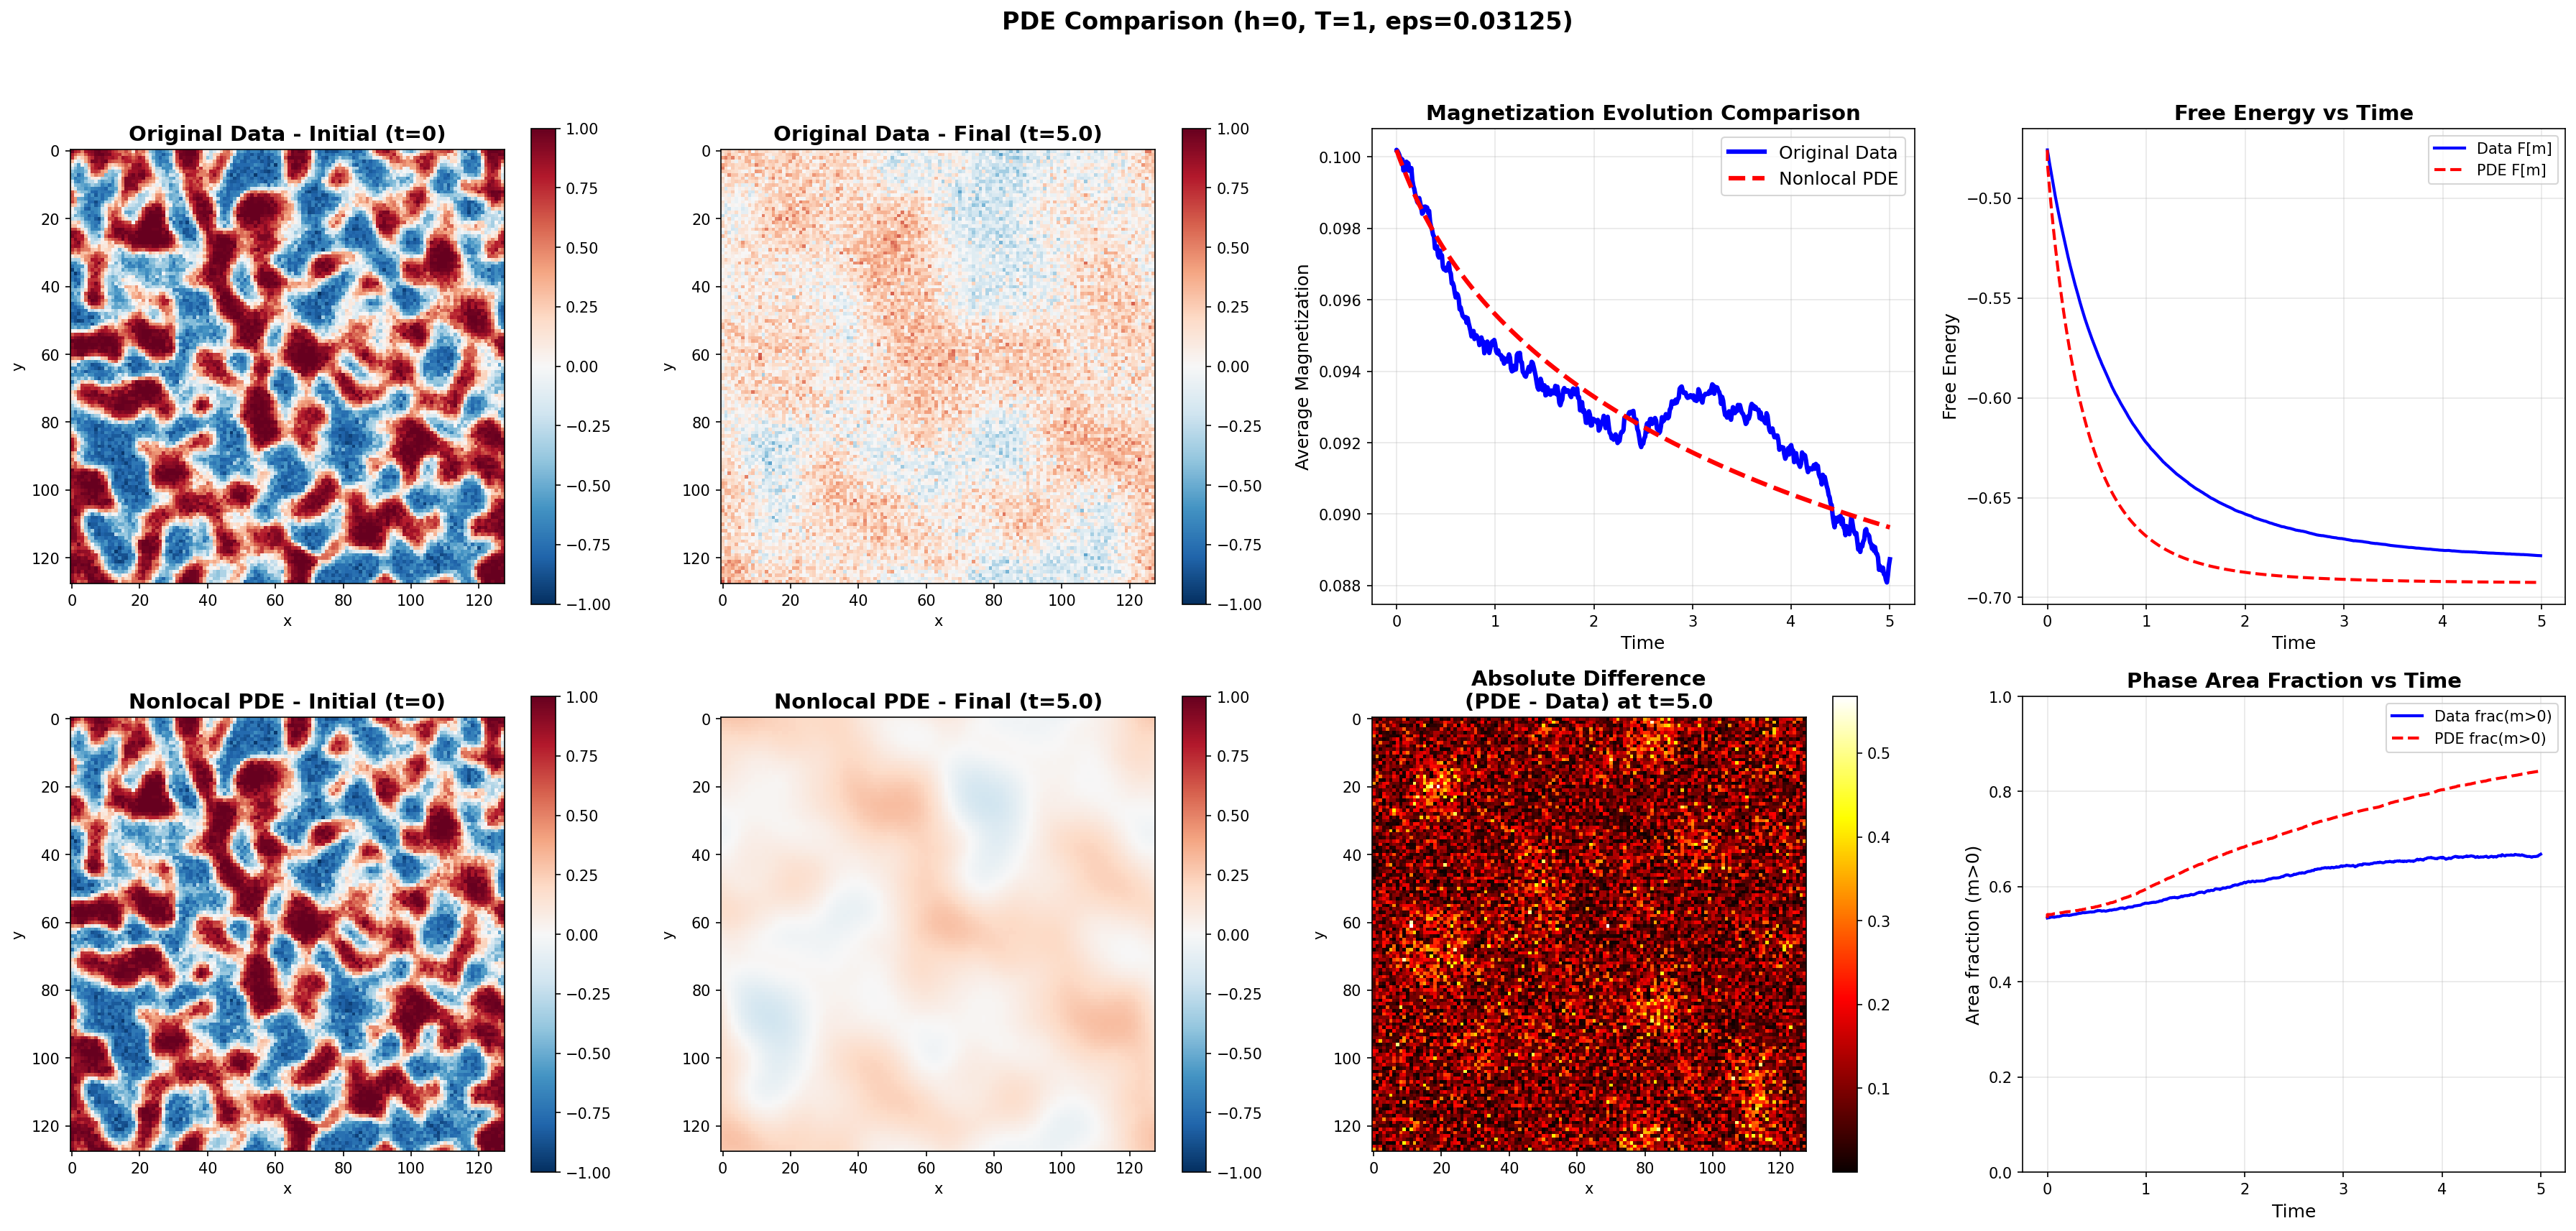
\includegraphics[width=1.0\textwidth]{fig/pde_comparison_h0_T1_eps0.03125.png}
    \caption{Comparison of original data and PDE solutions for $h=0$, $T=1$, $\epsilon=0.03125$.}
    \label{fig:pde_comparison_h0_T1_eps0.03125}
\end{figure}


\begin{figure}[h]
    \centering
    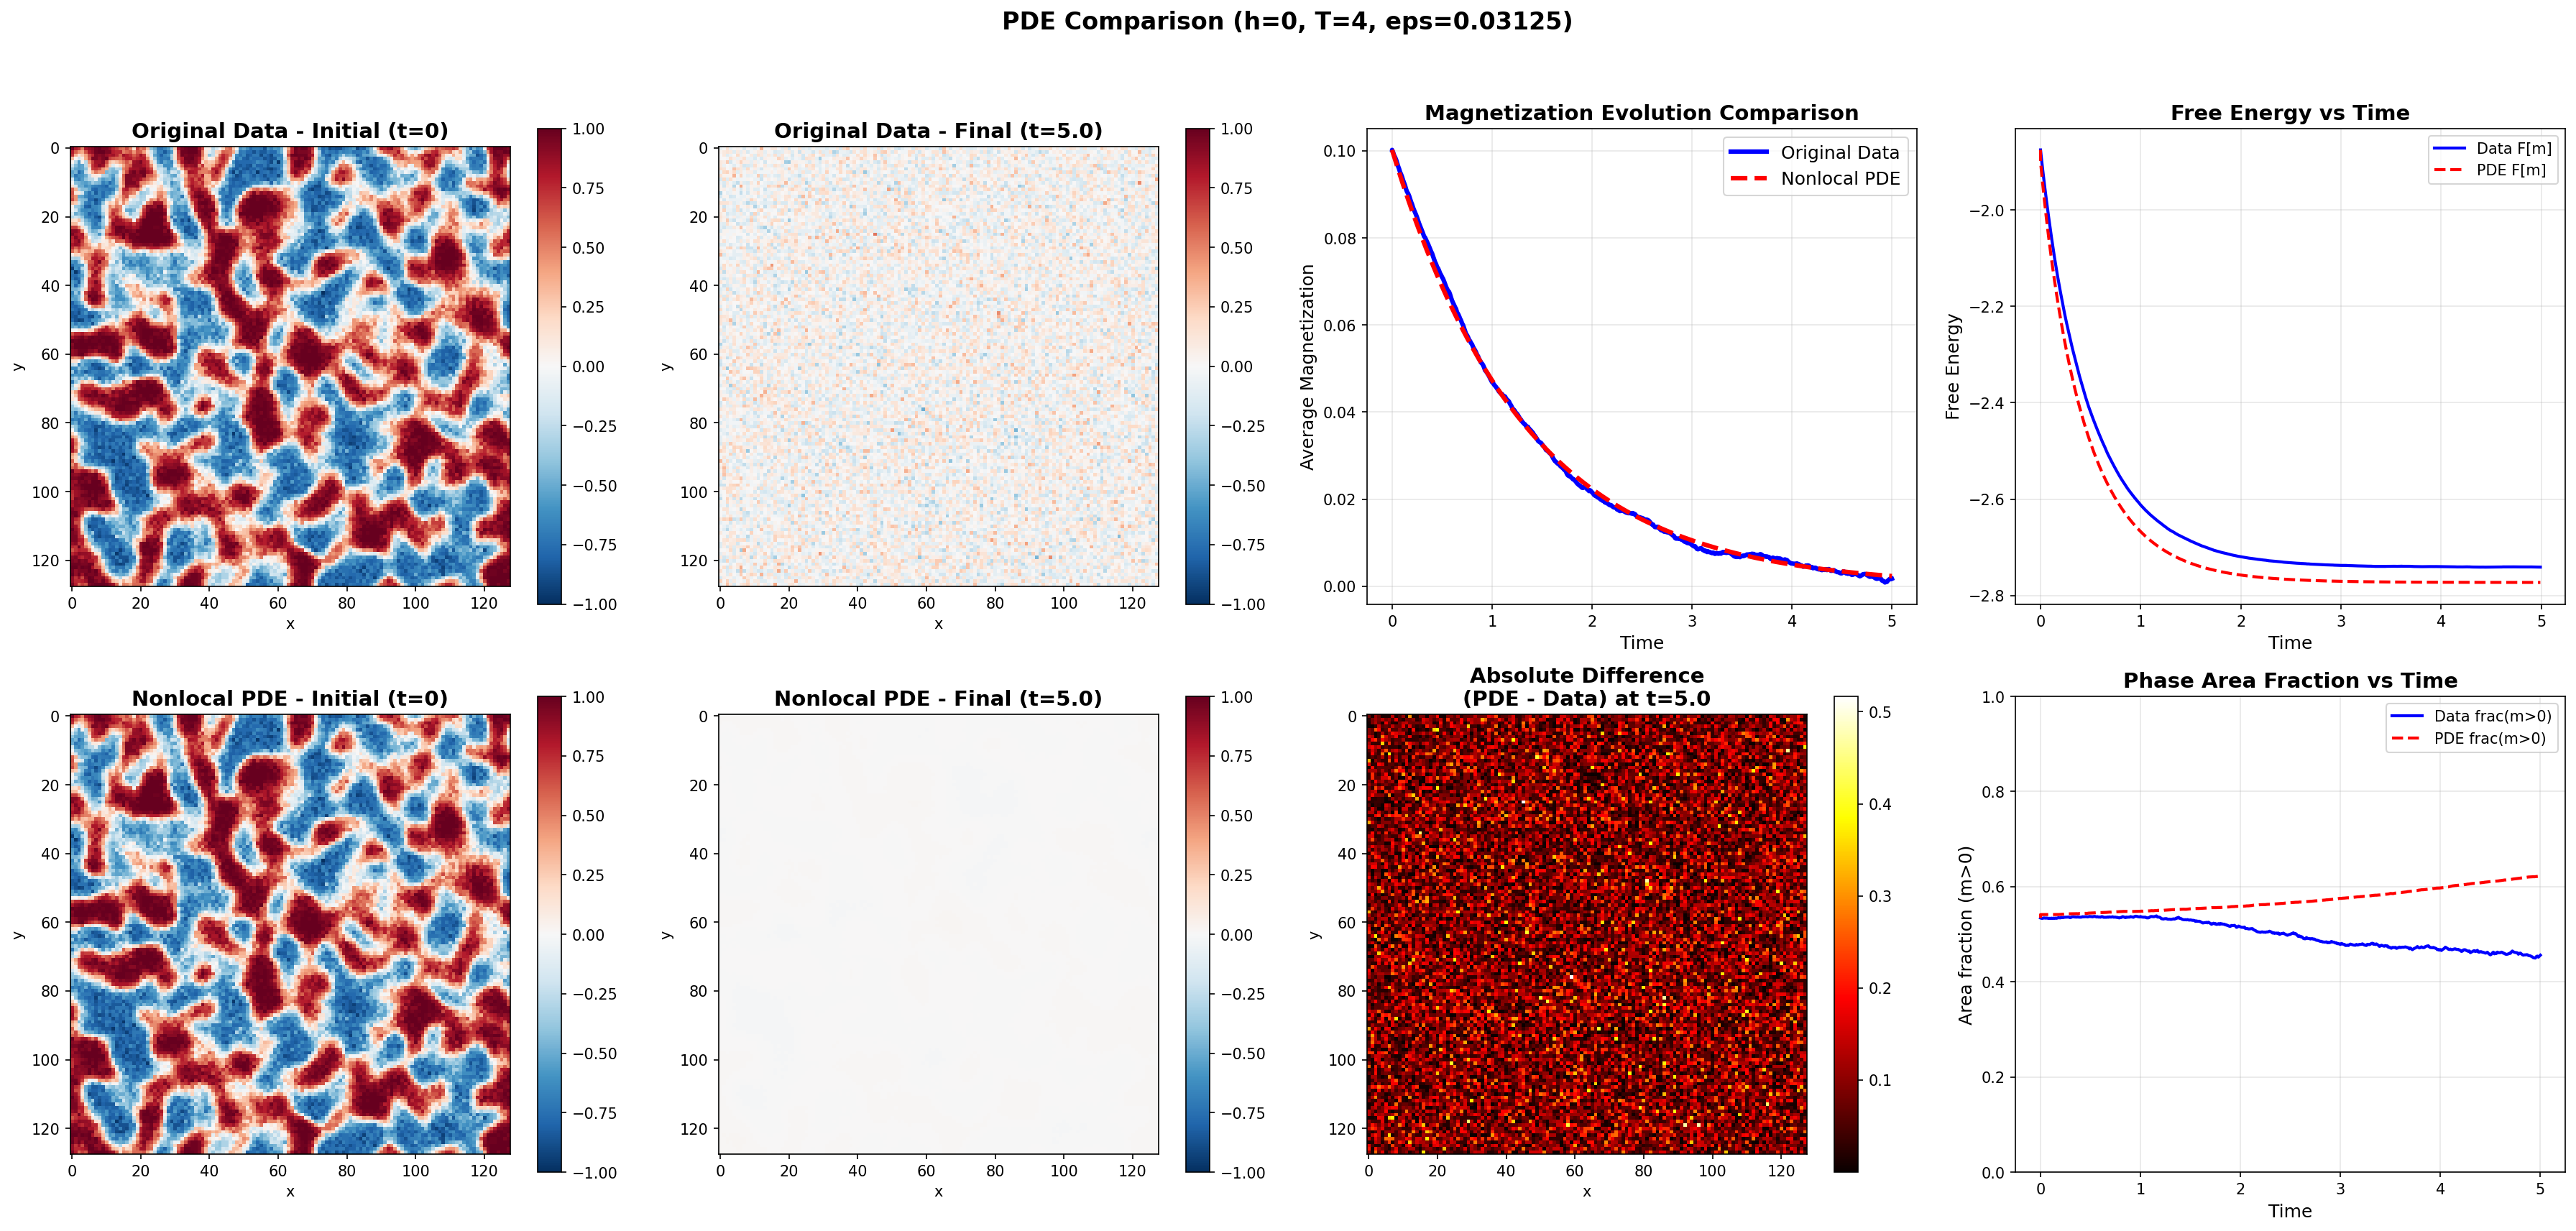
\includegraphics[width=1.0\textwidth]{fig/pde_comparison_h0_T4_eps0.03125.png}
    \caption{Comparison of original data and PDE solutions for $h=0$, $T=4$, $\epsilon=0.03125$.}
    \label{fig:pde_comparison_h0_T4_eps0.03125}
\end{figure}


\begin{figure}[!h]
    \centering
    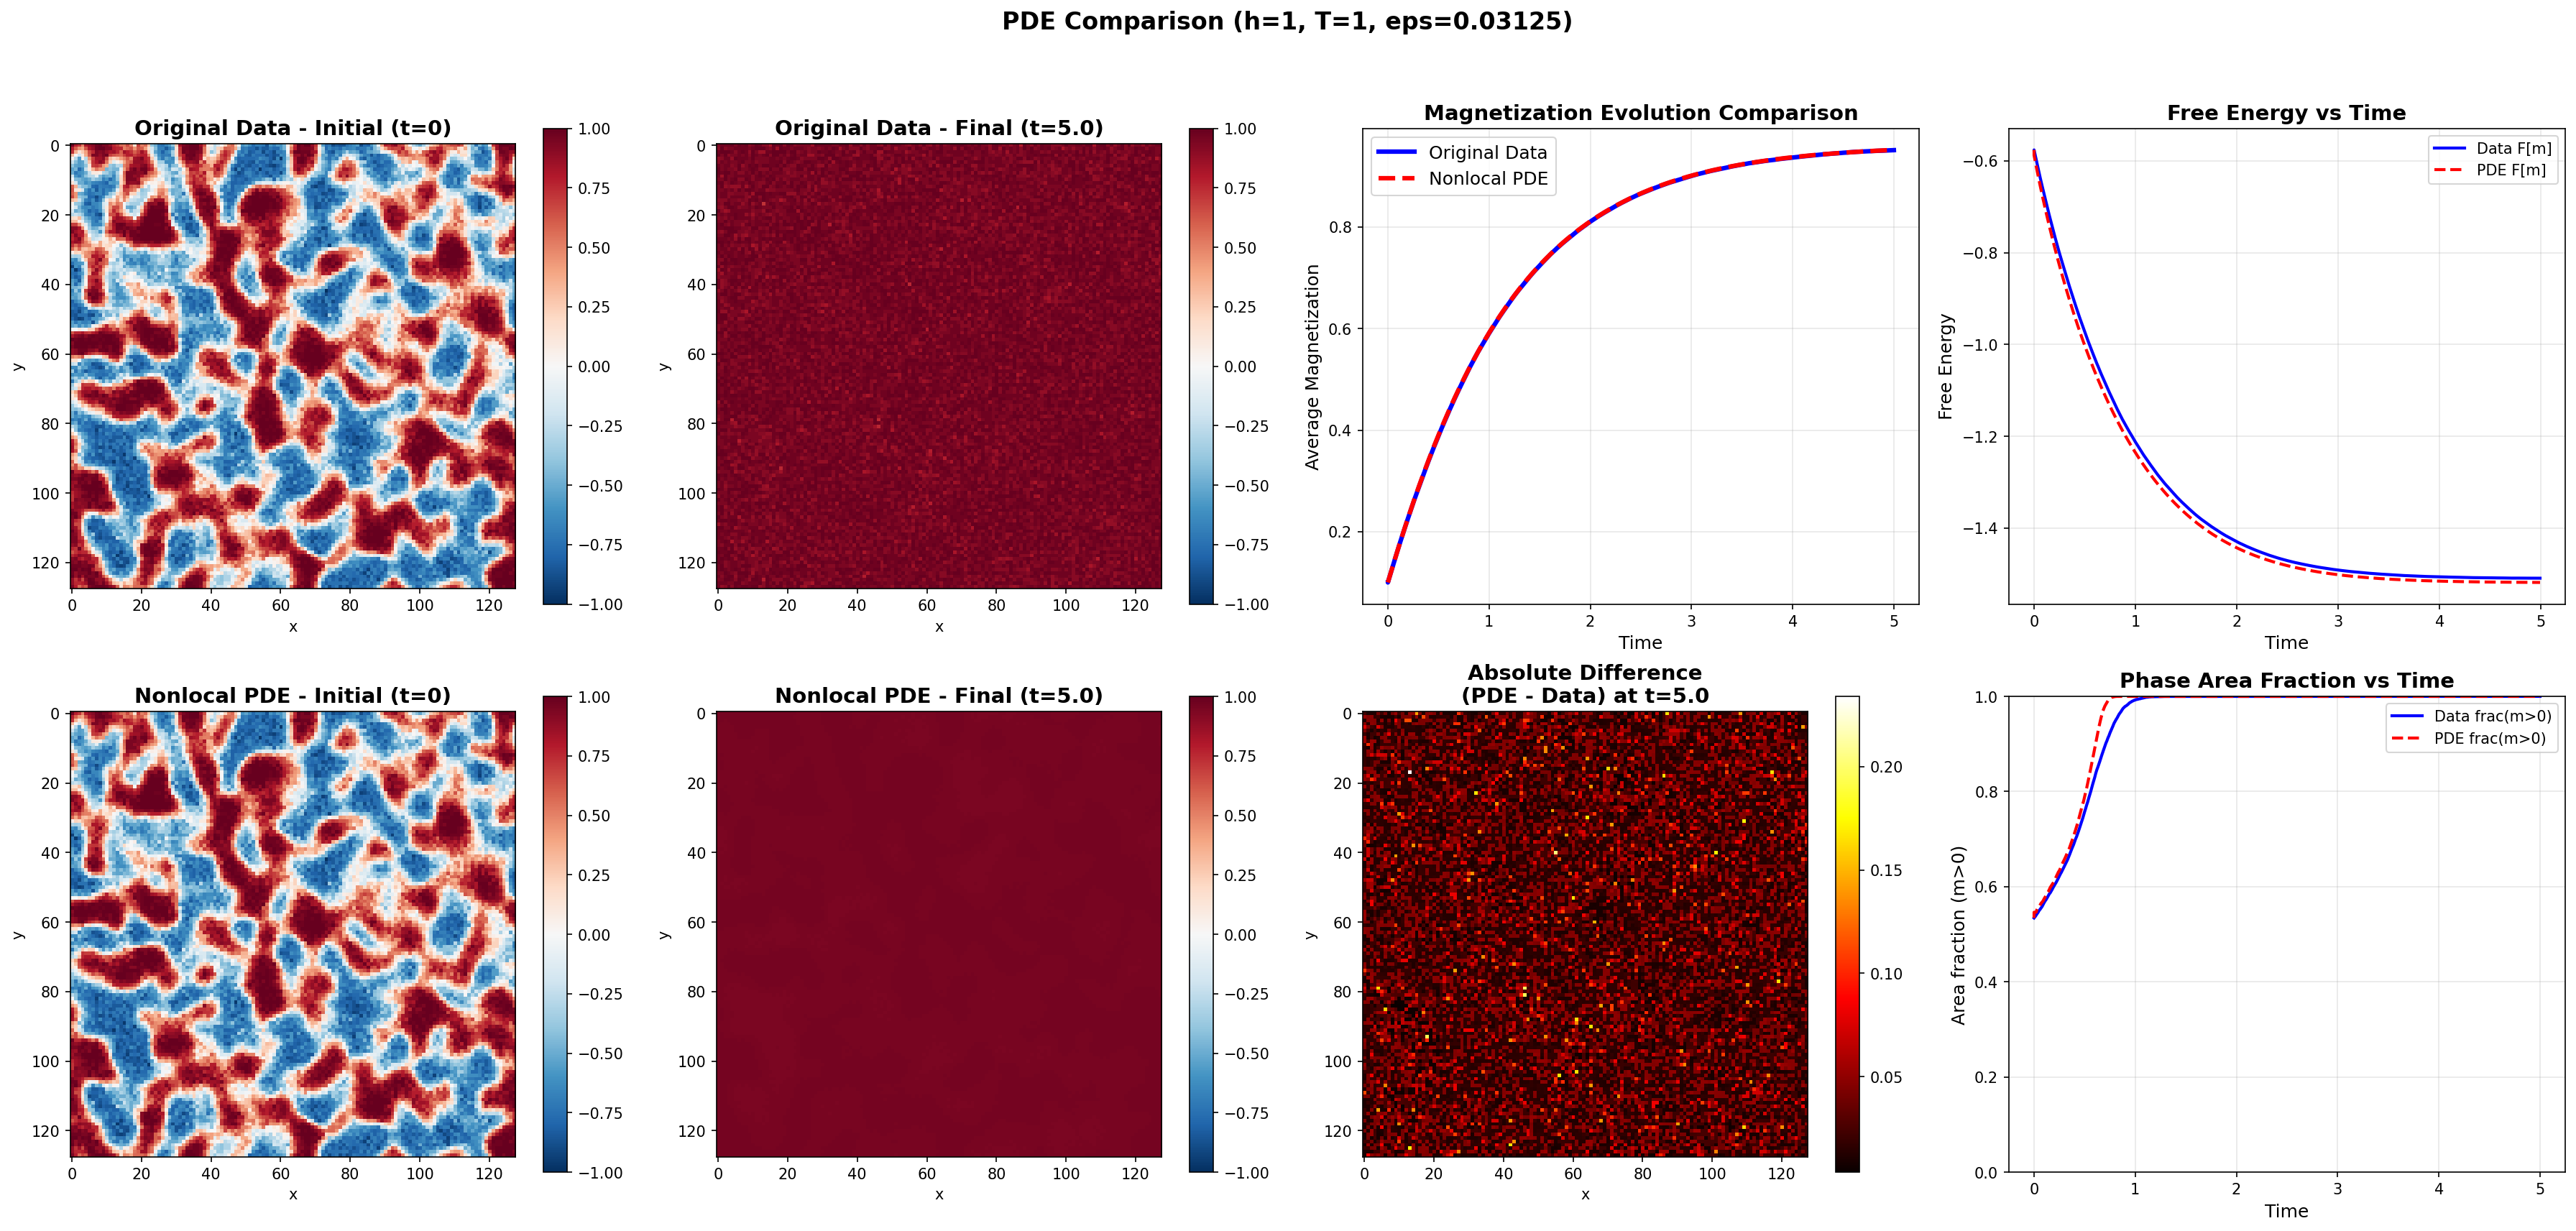
\includegraphics[width=1.0\textwidth]{fig/pde_comparison_h1_T1_eps0.03125.png}
    \caption{Comparison of original data and PDE solutions for $h=1$, $T=1$, $\epsilon=0.03125$.}
    \label{fig:pde_comparison_h1_T1_eps0.03125}
\end{figure}


\begin{figure}[h]
    \centering
    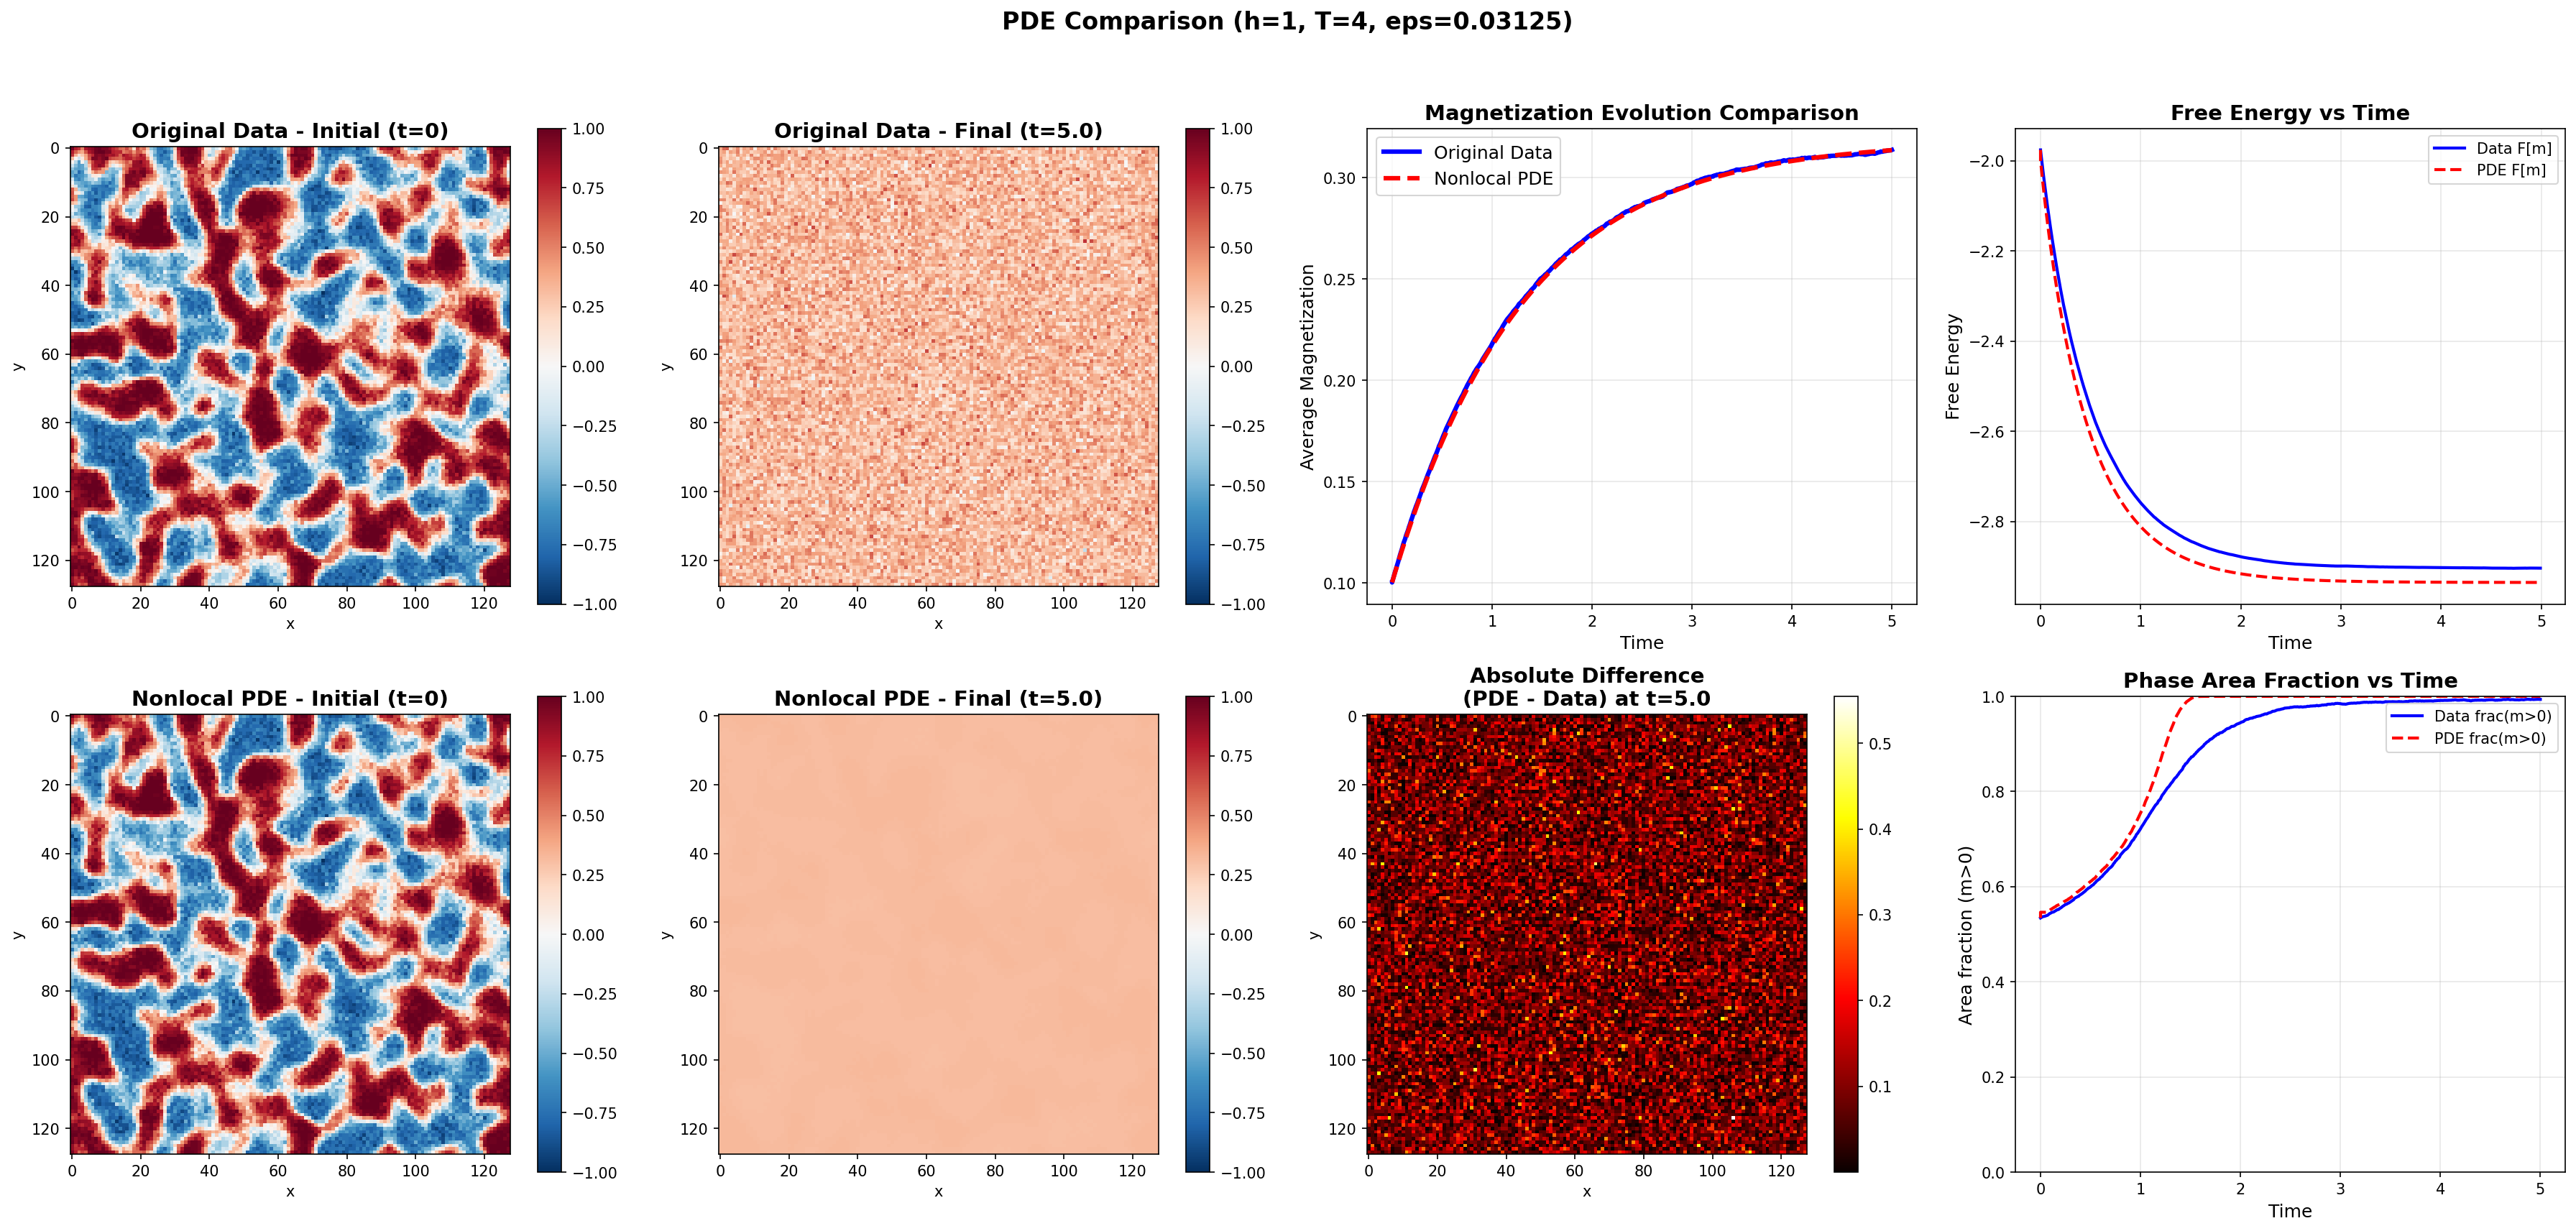
\includegraphics[width=1.0\textwidth]{fig/pde_comparison_h1_T4_eps0.03125.png}
    \caption{Comparison of original data and PDE solutions for $h=1$, $T=4$, $\epsilon=0.03125$.}
    \label{fig:pde_comparison_h1_T4_eps0.03125}
\end{figure}



\section{Network Training}

Recall that we want to train a network to predict the dynamics of the system.

\begin{equation}\label{eq:nonlocal-recall}
\partial_t m(t,x) \;=\; -\,m(t,x)\;+\;\tanh\!\Big(\beta\, (J_\gamma * m)(t,x) + \beta h\Big), \qquad m(0,x)=m_0(x),
\end{equation}



We have a generator parameterized like
\begin{equation}
    (\mathcal{L}m)(t,x) = F_\theta(I_\theta (m)(t,x), m(t,x))
\end{equation}

\begin{itemize}
    \item $m(.)$ can be a learned smooth function or $m_i$ itself; [-1, 1]
    \item $F_\theta(I,m)$ is $\mathbb{R}^2 \to \mathbb{R}$
    \begin{enumerate}
        \item Strong Prior: $F(I, m)=-Am+\tanh(\beta(BI+m+h))$; $F(I, m)=-Am+\tanh(BI+Cm+Dh))$, where $A,B,C,D$ are learnable parameters
        \item Weak Prior: an MLP with input size of 3 layers with hidden size of 128
    \end{enumerate}
    \item $I_\theta$ means we have a kernel $J_\theta$ to learn;
\end{itemize}


If the objective is to infer the interaction kernel J from data: 
(the obs part is obtained by difference? how we verify the learned structure?)

\begin{equation}
    J^\star, F^\star \;=\; \arg\min_{J, F}\;
\sum_{m \in \mathcal{D}}
\bigl\|\, \mathcal{L}(m;J,F)\;-\;\partial_t m_{\mathrm{obs}} \,\bigr\|_{L^2(\Omega)}^{2}.
\end{equation}


\nocite{*}
\printbibliography

\end{document}